

\title{\textbf{A Summary About My Work On CFG Matching}}

\author{
        Chen Chen 
}
\date{\today}

\documentclass[12pt]{article}
\usepackage{graphicx}
\usepackage{subfigure}

\begin{document}
\maketitle
* This is not a paper
\begin{abstract}
We noticed some good properties in CFG. For example, any CFG is or can be converted into a linear structure, besides, any node in CFG can be regarded as no more than two children( in fact, the case where a node has more than 2 children can be converted to several nodes with no more than 2 children). Therefore, we can abstract the CFG into some simplified graph by different levels, and comparing different CFGs in different abstraction levels is a very effective method to compare the similarity between them. We develop a algorithm for that and then prove its ability to be applied into any cases. We obey the rules not destroying the actual control flow throughout the whole algorithm, and it turns out working perfectly.
\end{abstract}

\section{Introduction}\

CFG matching is of great use in malware detecting nowadays. And traditional mathods are mainly about subgraphs. They are easy to understand and can work well under some circumstances. However, it would be hard for them when it comes to big graphs and they may work very slowly.\

In this paper, we proposed a novel method using abstraction conception. We first abstract the graph into a single node with a tree in it. And then we compare different CFGs by comparing the trees from the root level by level. 
\section{Algorithm}
\textbf{A. PRE-OPERATION:}\

As mentioned in ABSTRACT, there is a good and useful properties in CFG: Most CFGs have only one enter-point and one exit-node\\

   	 However, we have to admit that there exist some cases where that property are not satisfied. Thus, to ensure that following algorithm can be applied to any case, we have to do pre-operation:\\

\textit{\textbf{pre-operation}} It's true that each function has only one enter-node, but may not only one exit-node. However, since any function, no matter how many exit-nodes it has, will return to the very function who has called it, we can set a virtual exit-node for each function. In this way, we can deal with all the functions as if they have only one exit-point. After that, we can see the excuting control flows beautifully from the enterpoint to the exit-node. Then, we can abstract the graph into a single node without actually voilating the control flow.\\

\begin{figure}
\begin{center}
\begin{minipage}[c]{0.5\textwidth}
\centering
\subfigure[Before operation]{
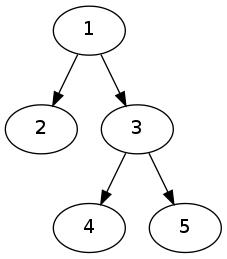
\includegraphics[width=0.4\textwidth]{cc3.jpg}}
\subfigure[After operation]{
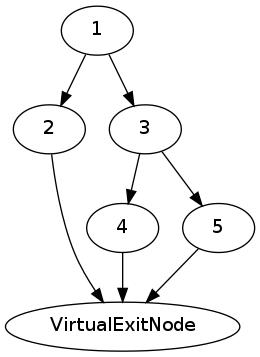
\includegraphics[width=0.4\textwidth]{cc4.jpg}}
\renewcommand{\figurename}{Figure}
\caption{Pre-operation method}
\label{}
\end{minipage}
\end{center}
\end{figure}

\textbf{B. ABSTRACTION METHOD:}\



There are three kinds of operation methods as follow:\\

    \textit{\textbf{abstraction method 1}} (1)Two subsequent nodes A(father) and B(child) can be abstracted into a single node if the the father node A has only one child(B) and the child B has only one  father(A); (2)  and if from node A two or more control flow branchs, which respectively point to node B1, B2 and so on (let's call them B-nodes), merge together to a single node C after leaving B-nodes, then we can simplify node A and B-nodes into one node, as the picture has showed in Figure 3.\
    
\begin{figure}[Htb]
\centering
\subfigure[Before method 1(1)]{
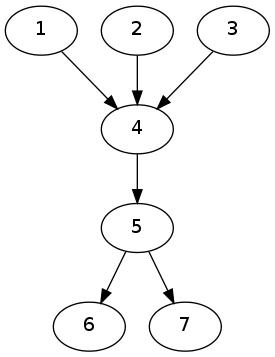
\includegraphics[width=0.2\textwidth]{cc5.jpg}}
\subfigure[After method 1(1)]{
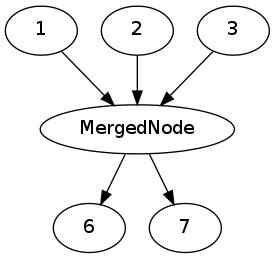
\includegraphics[width=0.2\textwidth]{cc6.jpg}}
\caption{Abstraction method 1(1)}
\subfigure[Before method 1(2)]{
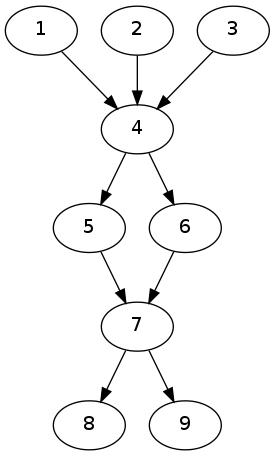
\includegraphics[width=0.2\textwidth]{cc7.jpg}}
\subfigure[After method 1(2)]{
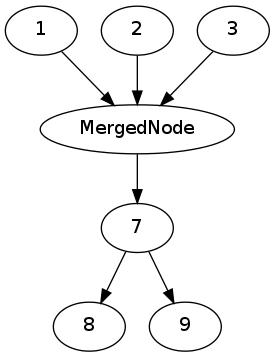
\includegraphics[width=0.2\textwidth]{cc8.jpg}}
\caption{Abstraction method 1(2)}
\end{figure}

\begin{figure}[!Htb]
\centering
\subfigure[Before method 2]{
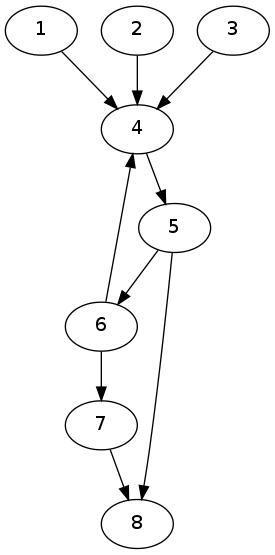
\includegraphics[width=0.2\textwidth]{cc9.jpg}}
\subfigure[After method 2]{
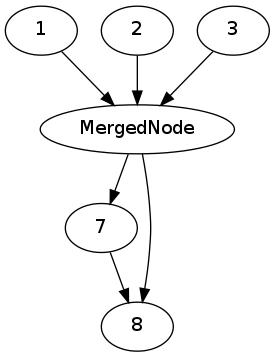
\includegraphics[width=0.2\textwidth]{cc10.jpg}}
\caption{Abstraction method 2}
\subfigure[Before method 3]{
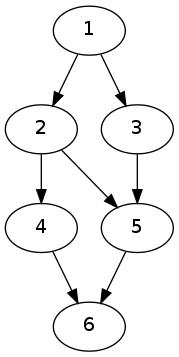
\includegraphics[width=0.2\textwidth]{cc11.jpg}}
\subfigure[After method 3]{
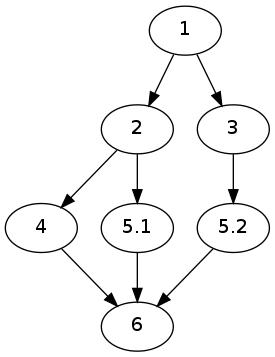
\includegraphics[width=0.2\textwidth]{cc12.jpg}}
\caption{Abstraction method 3}
\end{figure}


    \textit{\textbf{abstraction method 2}} All the nodes inside a loop can be simplified to a single node, and all the fathers and children are inherited by the created node. Since loops make the nodes inside them share the same control flow, this kind of abstraction does not conflict with the principle to reserve actual control flow.( About how to detect loops: we use a modified DFS to detect the loops in directed graph and it turns out working very well. However, since it's not the most crucial part of this algorithm, we will not illustrate it here.)\
    


    \textit{\textbf{abstraction method 3}} A node that has n other nodes pointing to can be replicated into n nodes which share the same offspring while have a single father. It's obvious that this way will not change the control flow.\\

\begin{figure}
\begin{center}
\begin{minipage}[c]{0.5\textwidth}
\centering
\subfigure[Before abstraction]{
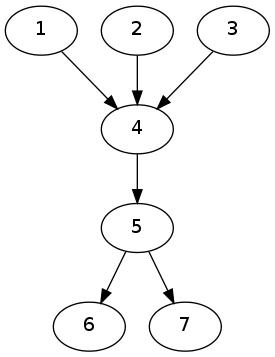
\includegraphics[width=0.4\textwidth]{cc5.jpg}}
\subfigure[After abstraction]{
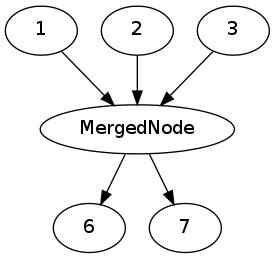
\includegraphics[width=0.4\textwidth]{cc6.jpg}}
\renewcommand{\figurename}{Figure}
\caption{Abstraction method 1(1) }
\label{}
\end{minipage}%
\begin{minipage}[c]{0.5\textwidth}
\centering
\subfigure[Before abstraction]{
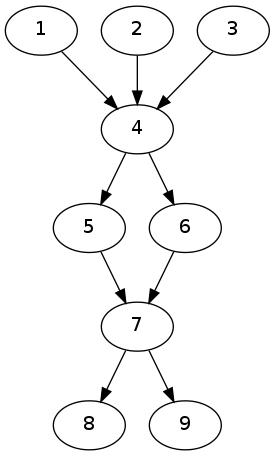
\includegraphics[width=0.4\textwidth]{cc7.jpg}}
\subfigure[After abstraction]{
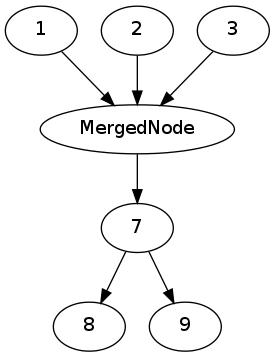
\includegraphics[width=0.4\textwidth]{cc8.jpg}}
\renewcommand{\figurename}{Figure}
\caption{Abstraction method 1(2)  }
\label{}
\end{minipage}
\end{center}
\end{figure}
    

Here is the algorithm about the order of pre-operations and abstraction methods:\\

\textbf{begin}\

\quad using pre-operation method 1 to modify CFG\

\quad using pre-operation method 2 to modify CFG\

\quad \textbf{Do While} CFG has been changed\

\qquad  \textbf{Do While} CFG has been changed\

\qquad \quad using abstraction method 1 to abstract CFG;\

\qquad \textbf{EndWhile}\

\qquad using abstraction method 2 to abstract CFG;\

\qquad using pre-operation method 1 to modify CFG;\

\quad \textbf{EndWhile}\

\quad \textbf{Do While} CFG has been changed\

\qquad \textbf{Do While} CFG has been changed\

\qquad \quad using abstraction method 1 to abstract CFG;\

\qquad \textbf{EndWhile}\

\qquad using abstraction method 3 to abstract CFG;\

\quad \textbf{EndWhile}\

\textbf{End}\\
\\               
\textbf{C. COMPARING METHOD:}\ 
  
To record the process of abstraction, we keep a tree in each node of the graph. Let's call the nodes in the tree as \textit{tnodes} in order to distinguish them with the nodes in the graph. There are also several properties in such tree and its tnodes:\\

\textbf{\textit{Property 1.}} Each tnode keeps two variable: NUM(int) and IFLOOP(bool). NUM records the number of leaves in this tnode's offspring, and IFLOOP shows whether there are loops in its offspring.  Those two variables are calculated when the tnode is created.\

\textbf{\textit{Property 2.}} If two nodes A and B are abstracted into one node C (there is already a tree in A with a root \textit{rootA}, and also a tree in B with \textit{rootB}), then as the first step to create a tree, we create a tnode(\textit{rootC}) in C as C's root, which has two children \textit{rootA} and \textit{rootB}. It should be noted that \textit{rootA} and \textit{rootB} should be kept in order as children(i.e. the bigger NUM is, the former the position in the ChildList), which is to avoid the obfuscation about the order in future comparison.And all the nodes as the offspring of \textit{rootA} and \textit{rootB} are copied into the new tree in C. NUM in \textit{rootC} is calculated by adding the NUM in \textit{rootA} with that in \textit{rootB}. And if either of the IFLOOPs in \textit{rootA} or \textit{rootB} is 1, the new IFLOOP in \textit{rootC} is 1. Similar actions happen when three nodes are abstracted(namely, a diamond is being abstracted).\\textit{Property 3.}

\textbf{\textit{Property 3.}} If more than three nodes are merged into a single node( namely, a loop is being abstracted),  we do similar thing with \textit{Property 2} except that the variable IFLOOP in the root of created node is set to 1.\\

After abstraction following the steps above, we can get a single most-abstracted node with a tree inside. Here comes to how we shall compare two different CFGs with such two nodes.\

* This has not been decided clearly yet, I think some parameter should be decided only after doing machine learning in order to ensure the best accuracy.\

* Of course, concerning the robustness, the comparing algorithm can be modified.\\
\\
\textbf{begin}\

\quad \textbf{If} the difference between the two NUMs in roots of the two CFGs is bigger than a set value \textbf{then}\

\qquad record that the two CFGs are not similar;\

\qquad exit;\

\quad \textbf{EndIf}\

\quad level := 1;\

\quad \textbf{While} level less than a set value \textbf{Do}\

\qquad \textbf{If} the number of the tnodes at current level is not the same \textbf{then}\

\qquad \quad record that the two CFGs are not similar;\

\qquad \quad exit;\

\qquad \textbf{Else}\

\qquad \quad \textbf{If} IFLOOP in the tnodes of current level is not same \textbf{then}\

\qquad \qquad record that the two CFGs are not similar;\

\qquad \qquad exit;\

\qquad \quad \textbf{Else}\

\qquad \qquad \textbf{If} the cosine similarity of  the two vectors composed by the NUMs in the tnodes of current level is less than a set value \textbf{then}\

\qquad \qquad \quad record that the two CFGs are not similar;\

\qquad \qquad \quad exit;\

\qquad \qquad \textbf{EndIf}\

\qquad \quad \textbf{EndIf}\

\qquad \textbf{EndIf}\

\qquad level :=  level + 1\

\quad \textbf{EndWhile}\

\quad record that they are similar\
\\
\textbf{End} \\


\section{DEMONSTRATION:}\

* I have not listed the detailed demonstration, here is only a brief description about the reasonable line of thinking.\\

\textit{\textbf{step 1 }}	We needn't to consider the existence of loops since we merge all the nodes in a loop as a single node. It's sure that every loop can be dealt with in that way. We only need to prove that our algorithm can be applied to CFGs with no loops inside.\

\textit{\textbf{step 2 }}	 First we demonstrate that a graph in which all the nodes (except the enter-point and the virtual exit-point) has only one father and no more than 2 children can be simplified.\

\textit{\textbf{step 3 }}	Then we demonstrate that all the graphs without loop can be converted to the graph described in 2.


\section{Conclusions}
Personally I think our final work should be composed of three parts: \textit{Algorithm}, \textit{Demonstration} and \textit{Testing}. And more work is needed after I go back to test this method.


\end{document}
This is never printed
